%--------------------------------------------------
\subsection{Prototipo 3: Integración de sistema de recomendación basado en filtrado colaborativo primera versión}
Dentro del análisis para el desarrollo de este prototipo se incorporan los siguientes requerimientos funcionales: \\
\begin{itemize}
	\item \hyperlink{RFSGPyPDR}{RFGPPR3 Generar módulo de recomendaciones basado el filtrado colaborativo.}
	\item \hyperlink{RFSGPyPDR}{RFGPPR22 Obtener recomendaciones globales}
	\item \hyperlink{RFSGPyPDR}{RFGPPR23 Obtener recomendaciones por departamento.}
\end{itemize}

definidos previamente en el capítulo del ``Bosquejo general de la aplicación''  con el título de ``Requerimientos funcionales del Sistema de Gestión, Procesamiento y Proveedor de Datos Retail''. \\ \par

\title{\textbf{Simbología necesaria:}
\\W := Matriz de pesos de los usuarios.
\\X := Matriz de pesos de productos.
\\p := valor de la predicción.
\\$ W^{(usuario)}$ := Vector de pesos de un usuario.
\\$ X^{(producto)}$ := Vector de pesos de un producto.
\\$ y^{(i,j)}$ := Calificación para el producto i hecha por el usuario j. 
\\$ r(i,j) = 1$ := Producto i calificado por usuario j.\\
%--------------------------------------------------
\subsubsection{Análisis}
Durante esta sección se explicarán algunos de los elementos del algoritmo Filtrado Colaborativo comenzando con el diagrama de flujo de dicho algoritmo que se muestra en la figura \ref{diagrama_flujo_filtrado_colaborativo}

\FloatBarrier
\begin{figure}[htbp!]
		\centering
			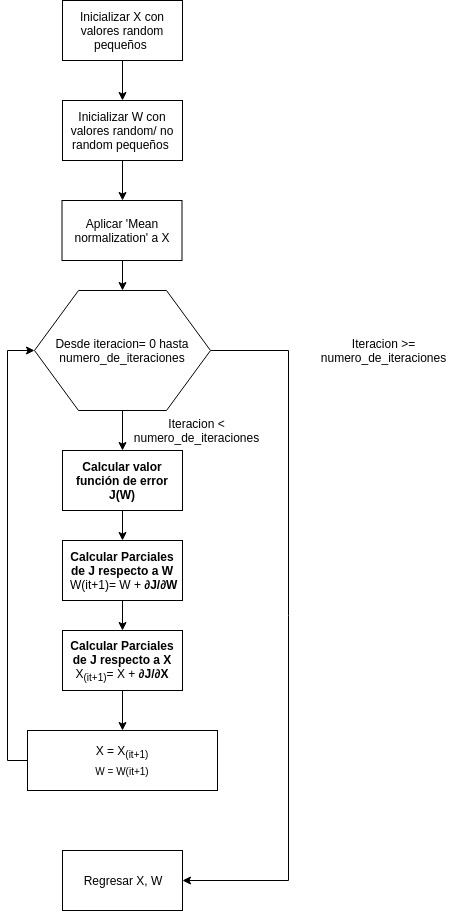
\includegraphics[width=0.6 \textwidth]{imagenes/sistemarec/algoritmo_sistema}
		\caption{Diagrama de flujo de algoritmo Filtrado Colaborativo.}
		\label{diagrama_flujo_filtrado_colaborativo}
\end{figure}
\FloatBarrier


\textbf{\\Predicción de calificación por usuario}\\
La calificación predicha de cada producto para cierto usuario se define de la siguiente manera:
\begin{equ}[!ht]
  \begin{equation}
	p = {W^{usuario}}^{T}X^{producto}
  \end{equation}
 \caption{Definición matemática de la predicción de un producto.}
  \label{equation:hiperplano}
\end{equ}
\FloatBarrier
Esta ecuación significa lo siguiente: producto punto del vector de pesos de un usuario por el vector de pesos de cada producto.
\\\\\textbf{Función de error}\\
La función de error seleccionada para este algoritmo se llama \textbf{Error cuadrático medio}. Esta medida se seleccionó porque por cada error cometido por el modelo éste se penaliza de una manera cuadrática además de tener una representación gráfica muy simple y lógica. 
\begin{equ}[!ht]
  \begin{equation}
  \begin{array}{c}
	J = \frac{1}{num.productos} \sum_{i}^{num.productos} \sum_{j}^{num.usuarios} ({W^{(j)}}^{T}X^{(i)} - y^{(i,j)})^2
  \end{array}
  \end{equation}
 \caption{Definición matemática de la función de error.}
  \label{equation:J}
\end{equ}
\FloatBarrier
%%%%%%%%%%%%%%%%%%%%%%%%%%%%%
\textbf{\\Gradiente descendiente}\\
Esta técnica se utiliza para encontrar el mínimo de una función aproximando éste de una manera numérica, como lo dice su nombre se hace encontrando la taza de cambio de J respecto a una variable (en el caso de Filtrado Colaborativo respecto a W y X) $ \frac{\partial(J)}{\partial(W)} $ y $ \frac{\partial(J)}{\partial(X)} $, ya que, hay que minimizar el error de J respecto a dichas variables. \\
Finalmente, en la figura \ref{gradiente_desc} se puede visualizar una representación gráfica en dos dimesiones de lo que hace el algoritmo.

\FloatBarrier
\begin{figure}[htbp!]
		\centering
			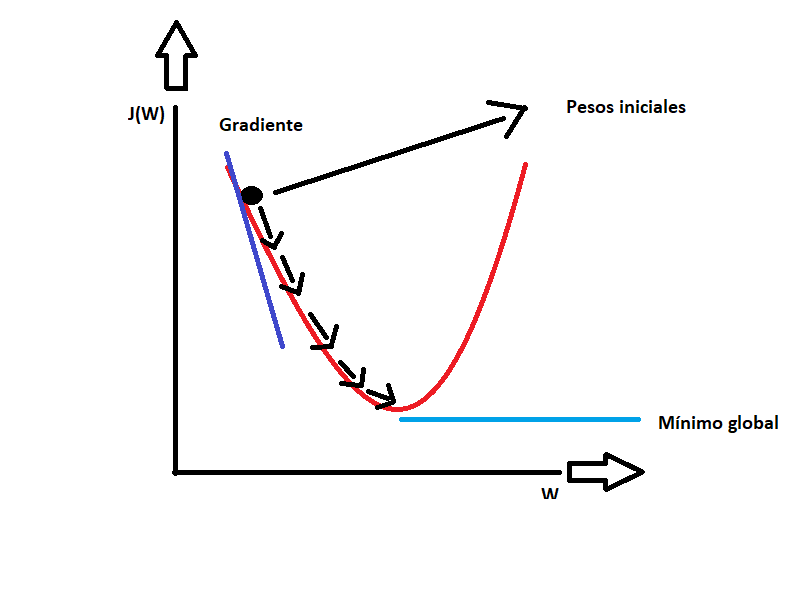
\includegraphics[width=0.6 \textwidth]{imagenes/sistemarec/gradiente_descendiente}
		\caption{Gradiente descendiente.}
		\label{gradiente_desc}
\end{figure}
\FloatBarrier

\textbf{\\Gradiente de J respecto a W ( $ \frac{\partial(J)}{\partial(W)} $ )}\\
Como se mencionó en la sección de Gradiente descendiente una de las variables respecto a las cuáles se tiene que minimizar J es W, esto significa ajustar los Pesos de los usuarios de tal manera que J sea cada vez menor y por lo tanto lograr una generalización consistente con los datos. Esto se expresa de la siguiente manera:

\begin{equ}[!ht]
  \begin{equation}
  \begin{array}{c}
	W^{(j)} = W^{(j)} - \alpha \sum_{i:r(i,j) = 1} (({W^{j}}^T X^{(i)} - y^{(i,j)}))X^{(i)}  
  \end{array}
  \end{equation}
 \caption{Definición matemática del gradiente respecto a W.}
  \label{equation:gradw}
\end{equ}
\FloatBarrier
Como se puede observar en la ecuación \ref{equation:gradw} se hace la actualización de $W^{(i)}$ restando un termino, este termino es el gradiente multiplicado por un coeficienite de aprendizaje ($\alpha$) que establece el tamaño del movimiento hacía el mínimo.
\\\\\textbf{Gradiente de J respecto a X ( $ \frac{\partial(J)}{\partial(X)} $ )}\\
Como se mencionó en la sección de Gradiente descendiente la otra variable a minimizar J es X, esto significa ajustar los Pesos de los productos de tal manera que J sea cada vez menor y por lo tanto lograr una generalización consistente con los datos. Esto se expresa de la siguiente manera:

\begin{equ}[!ht]
  \begin{equation}
  \begin{array}{c}
	X^{(i)} = X^{(i)} - \alpha \sum_{i:r(i,j) = 1} (({W^{j}}^T X^{(i)} - y^{(i,j)}))W^{(j)}  
  \end{array}
  \end{equation}
 \caption{Definición matemática del gradiente respecto a X.}
  \label{equation:gradw}
\end{equ}
\FloatBarrier
Como se puede observar en la ecuación \ref{equation:gradw} se hace la actualización de $W^{(i)}$ restando un termino, este termino es el gradiente multiplicado por un coeficienite de aprendizaje ($\alpha$) que establece el tamaño del movimiento hacía el mínimo.
\\\\\title{\textbf{Aplicar Mean normalization a X}\\\\
\textit{Este algoritmo es explicado y aplicado en el siguiente prototipo.} 

%--------------------------------------------------
\subsubsection{Diseño}

%%%%%%%%%%%%%%%%%%%%%%%%%%%%%%%%%%%%%%%%%%%%%%%%%%%%%%%%%%%%%%%
\title{\textbf{RFGPPR22 Obtener recomendaciones globales}
\begin{itemize}
\item Ruta: /client/get-global-recom/{id\_usuario}
\begin{itemize}
\item Método: GET
\item Tipo de parámetro: ruta
\item Opciones [id\_usuario, int]
\item Respuesta exitosa:
\begin{lstlisting}[language=json,firstnumber=1]
{	"products": [{
		"id_producto" : integer,
		"producto": "string",
		"precio_venta" : "string",
		"stock" : integer,
		"departamento" : "string",
		"tienda" : "string",
		"categoria" : "string",
		"marca" : "string",
		"promocion" : "string",
		"imagen": "string"
		"score" : float
},
{...},
{...},
...]}
\end{lstlisting}

\item Respuesta erronea:
\begin{lstlisting}[language=json,firstnumber=1]
{
    "message": "string",
}
\end{lstlisting}
\end{itemize}
\end{itemize}

%%%%%%%%%%%%%%%%%%%%%%%%%%%%%%%%%%%%%%%%%%%%%%%%%%%%%%%%%%%%%%%%%%
\title{\textbf{RFGPPR23 Obtener recomendaciones por departamento.}
\begin{itemize}
\item Ruta: /client/recommendations/department/(id\_usuario)/{id\_departamento}
\begin{itemize}
\item Método: GET
\item Tipo de parámetro: ruta
\item Opciones [id\_usuario, int], [id\_departamento, int]
\item Respuesta exitosa:
\begin{lstlisting}[language=json,firstnumber=1]
{	"products": [{
		"id_producto" : integer,
		"producto": "string",
		"precio_venta" : "string",
		"stock" : integer,
		"departamento" : "string",
		"tienda" : "string",
		"categoria" : "string",
		"marca" : "string",
		"promocion" : "string",
		"imagen": "string"
		"score" : float
},
{...},
{...},
...]}
\end{lstlisting}

\item Respuesta erronea:
\begin{lstlisting}[language=json,firstnumber=1]
{
    "message": "string",
}
\end{lstlisting}
\end{itemize}
\end{itemize}

\subsubsection{Pruebas}
\textit{Las pruebas del sistema fueron hechas sobre una laptop Lenovo Thinkpad T460 con las siguientes carácteristicas:\\}
\begin{itemize}
\item Procesador Intel® Core™ i5-5300U (3M Cache, hasta 2,90 GHz).
\item 8 GB RAM.
\item 240 GB Solid State Drive ROM.
\item Sistema Operativo Fedora 27.
\end{itemize}
%%%%%%%%%%%%%%%%%%%%% PRUEBA 1
\title{\textbf{Prueba 1.}}

\begin{itemize}
\item Número de clientes:184
\item Número de productos: 10001
\item Número de compras: 144192
\item Número de iteraciones: 30
\item Número de parámetros: 23
\item Tasa de aprendizaje: 0.01
\end{itemize}

\textbf{Prueba con validación: 70\% entrenamiento 30\% validación}

\FloatBarrier
\begin{figure}[htbp!]
		\centering
			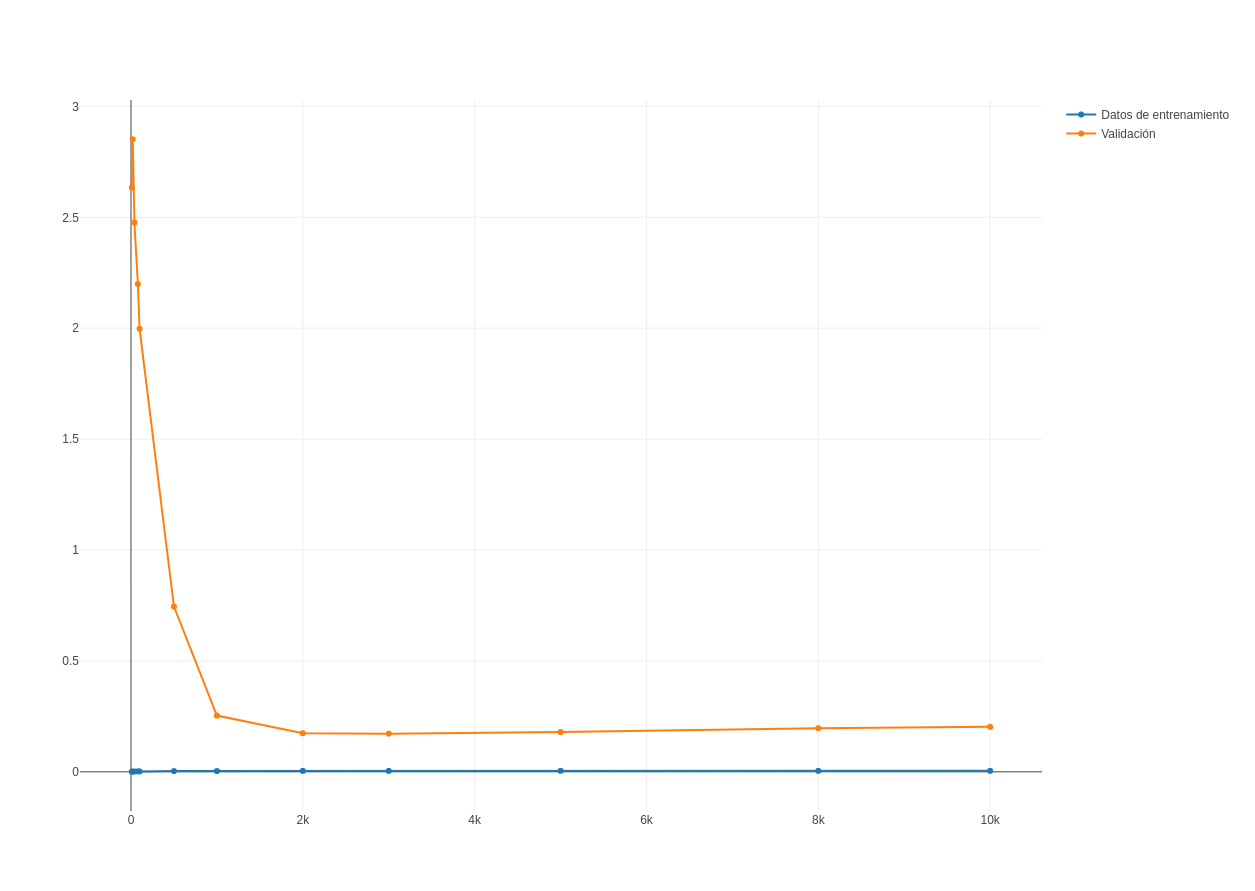
\includegraphics[width=1 \textwidth]{imagenes/pruebassistemarecom/30_0_23}
		\caption{Prueba 1 con validación.}
\end{figure}
\FloatBarrier
\newpage
\textbf{Prueba de J respecto al número de iteraciones}

\FloatBarrier
\begin{figure}[htbp!]
		\centering
			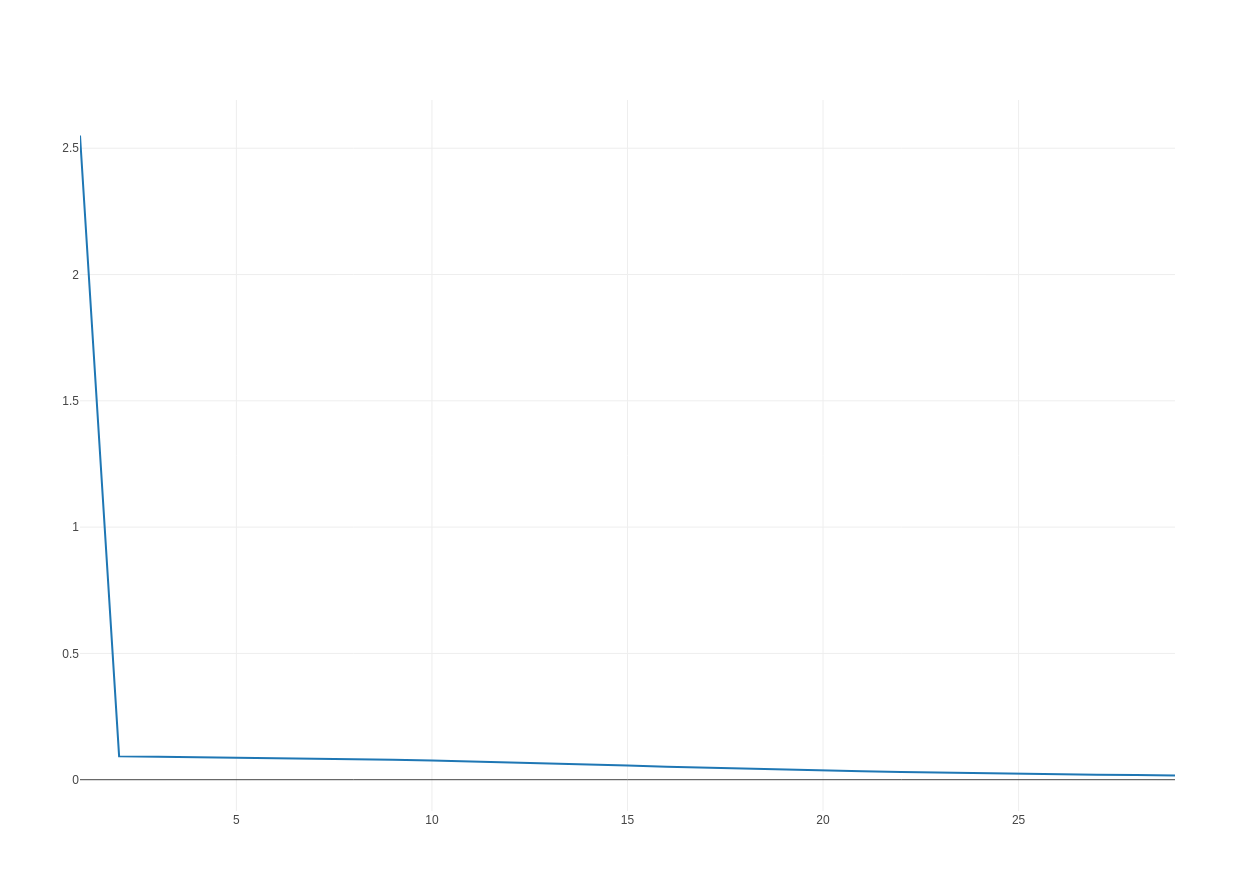
\includegraphics[width=1 \textwidth]{imagenes/pruebassistemarecom/1_j}
		\caption{Prueba 1: J respecto al número de iteraciones.}
\end{figure}
\FloatBarrier

%%%%%%%%%%%%%%%%%%%%% PRUEBA 2
\title{\textbf{Prueba 2.}}

\begin{itemize}
\item Número de clientes:184
\item Número de productos: 10001
\item Número de compras: 144192
\item Número de iteraciones: 15
\item Número de parámetros: 13
\item Tasa de aprendizaje: 0.01
\end{itemize}
\newpage
\textbf{Prueba con validación: 70\% entrenamiento 30\% validación}

\FloatBarrier
\begin{figure}[htbp!]
		\centering
			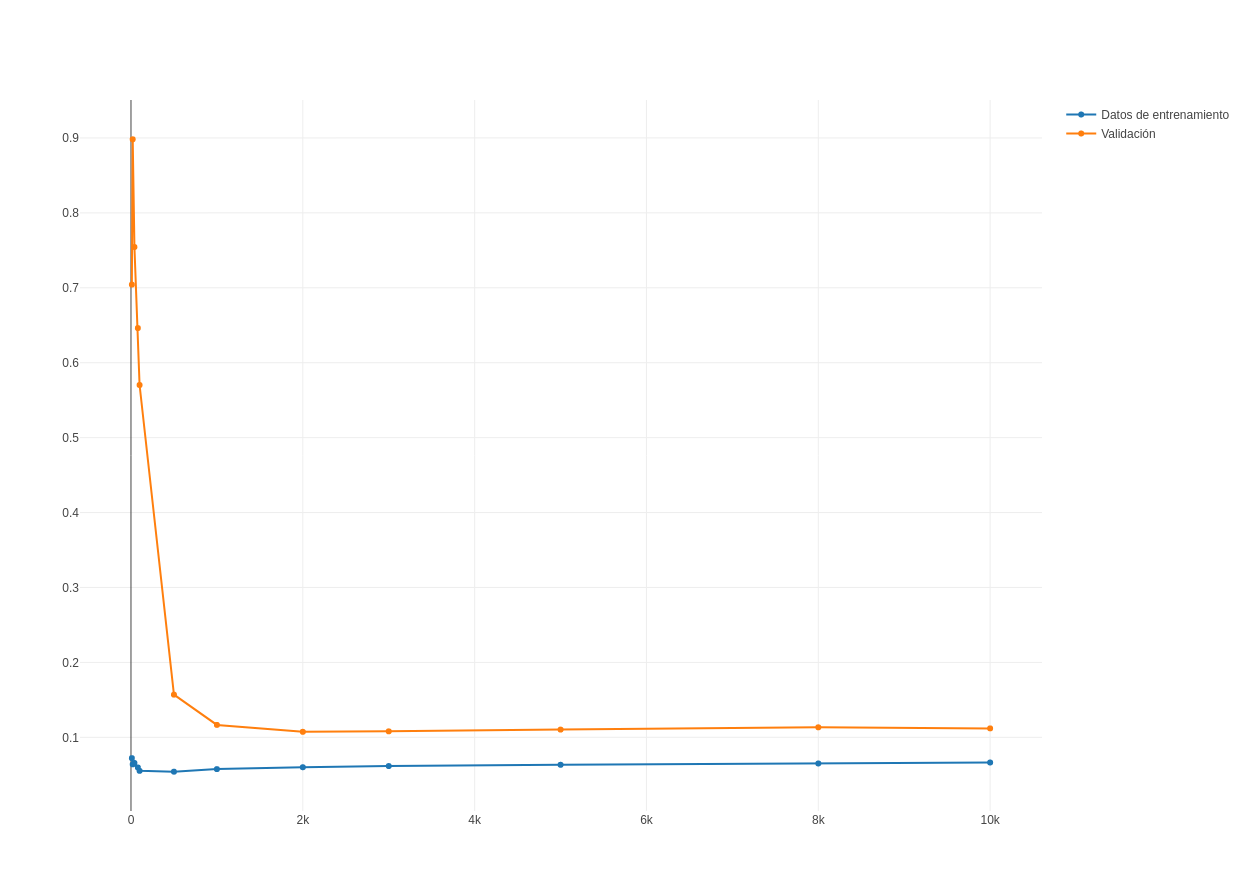
\includegraphics[width=1 \textwidth]{imagenes/pruebassistemarecom/15_0_13}
		\caption{Prueba 2 con validación.}
\end{figure}
\FloatBarrier
\newpage
\textbf{Prueba de J respecto al número de iteraciones}

\FloatBarrier
\begin{figure}[htbp!]
		\centering
			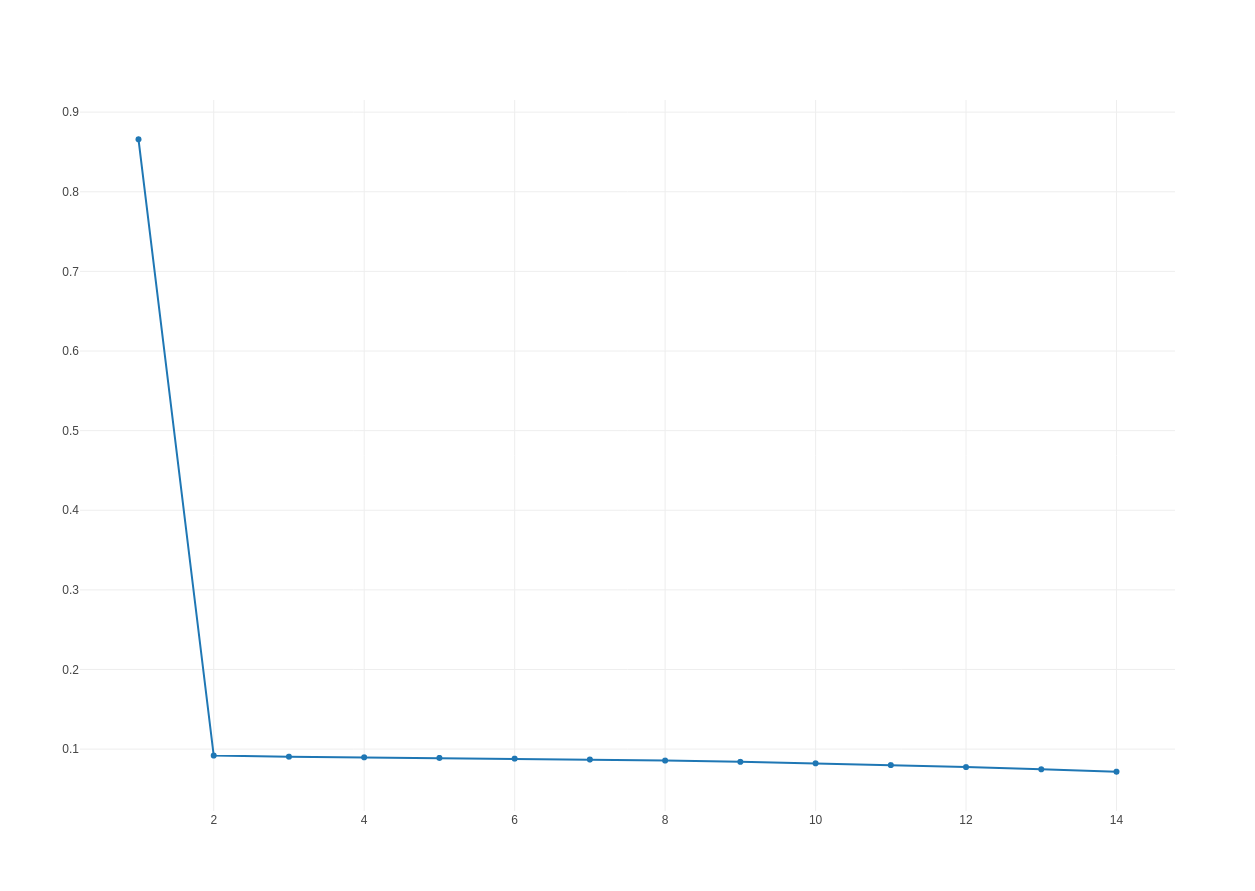
\includegraphics[width=1 \textwidth]{imagenes/pruebassistemarecom/2_j}
		\caption{Prueba 2: J respecto al número de iteraciones.}
\end{figure}
\FloatBarrier

%%%%%%%%%%%%%%%%%%%%% PRUEBA 3
\title{\textbf{Prueba 3.}}

\begin{itemize}
\item Número de clientes:184
\item Número de productos: 10001
\item Número de compras: 144192
\item Número de iteraciones: 5
\item Número de parámetros: 13
\item Tasa de aprendizaje: 0.01
\end{itemize}
\newpage
\textbf{Prueba con validación: 70\% entrenamiento 30\% validación}

\FloatBarrier
\begin{figure}[htbp!]
		\centering
			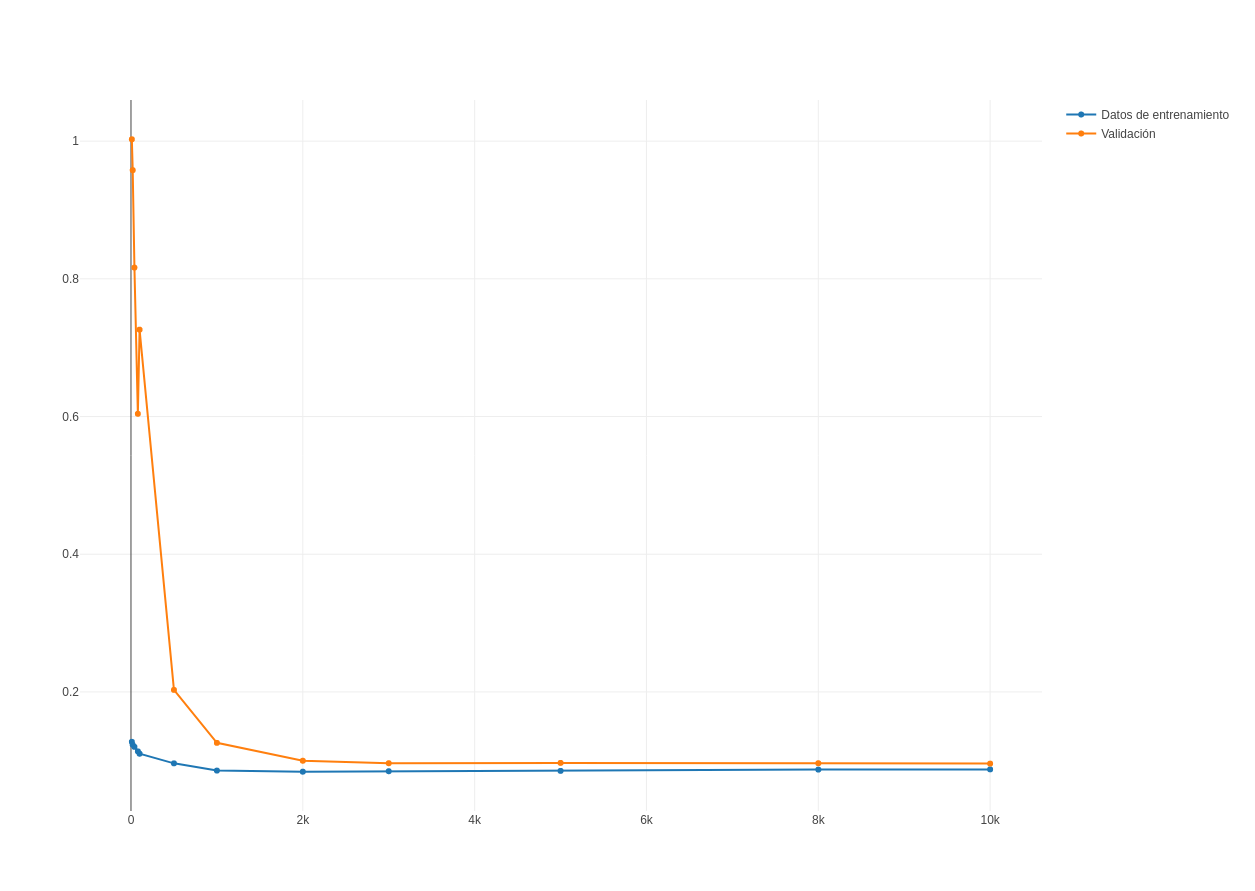
\includegraphics[width=1 \textwidth]{imagenes/pruebassistemarecom/5_0_13}
		\caption{Prueba 3 con validación.}
		\label{pruebabien}
\end{figure}
\FloatBarrier
\newpage
\textbf{Prueba de J respecto al número de iteraciones}

\FloatBarrier
\begin{figure}[htbp!]
		\centering
			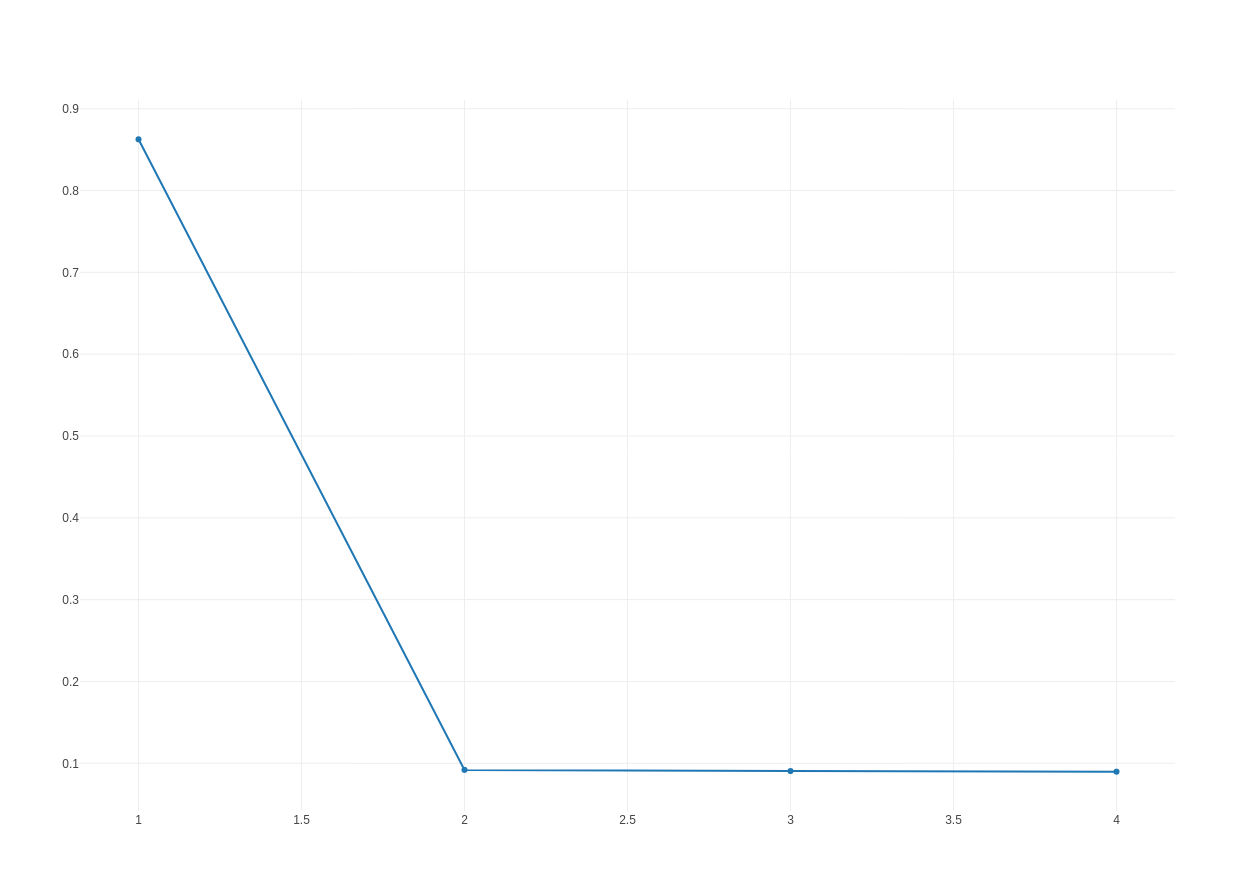
\includegraphics[width=1 \textwidth]{imagenes/pruebassistemarecom/3_j}
		\caption{Prueba 3: J respecto al número de iteraciones.}
\end{figure}
\FloatBarrier

